\documentclass[]{book}
\usepackage{lmodern}
\usepackage{amssymb,amsmath}
\usepackage{ifxetex,ifluatex}
\usepackage{fixltx2e} % provides \textsubscript
\ifnum 0\ifxetex 1\fi\ifluatex 1\fi=0 % if pdftex
  \usepackage[T1]{fontenc}
  \usepackage[utf8]{inputenc}
\else % if luatex or xelatex
  \ifxetex
    \usepackage{mathspec}
  \else
    \usepackage{fontspec}
  \fi
  \defaultfontfeatures{Ligatures=TeX,Scale=MatchLowercase}
\fi
% use upquote if available, for straight quotes in verbatim environments
\IfFileExists{upquote.sty}{\usepackage{upquote}}{}
% use microtype if available
\IfFileExists{microtype.sty}{%
\usepackage{microtype}
\UseMicrotypeSet[protrusion]{basicmath} % disable protrusion for tt fonts
}{}
\usepackage[margin=1in]{geometry}
\usepackage{hyperref}
\hypersetup{unicode=true,
            pdftitle={Intermediate Macroeconomics},
            pdfauthor={François Geerolf},
            pdfborder={0 0 0},
            breaklinks=true}
\urlstyle{same}  % don't use monospace font for urls
\usepackage{natbib}
\bibliographystyle{apalike}
\usepackage{longtable,booktabs}
\usepackage{graphicx,grffile}
\makeatletter
\def\maxwidth{\ifdim\Gin@nat@width>\linewidth\linewidth\else\Gin@nat@width\fi}
\def\maxheight{\ifdim\Gin@nat@height>\textheight\textheight\else\Gin@nat@height\fi}
\makeatother
% Scale images if necessary, so that they will not overflow the page
% margins by default, and it is still possible to overwrite the defaults
% using explicit options in \includegraphics[width, height, ...]{}
\setkeys{Gin}{width=\maxwidth,height=\maxheight,keepaspectratio}
\IfFileExists{parskip.sty}{%
\usepackage{parskip}
}{% else
\setlength{\parindent}{0pt}
\setlength{\parskip}{6pt plus 2pt minus 1pt}
}
\setlength{\emergencystretch}{3em}  % prevent overfull lines
\providecommand{\tightlist}{%
  \setlength{\itemsep}{0pt}\setlength{\parskip}{0pt}}
\setcounter{secnumdepth}{5}
% Redefines (sub)paragraphs to behave more like sections
\ifx\paragraph\undefined\else
\let\oldparagraph\paragraph
\renewcommand{\paragraph}[1]{\oldparagraph{#1}\mbox{}}
\fi
\ifx\subparagraph\undefined\else
\let\oldsubparagraph\subparagraph
\renewcommand{\subparagraph}[1]{\oldsubparagraph{#1}\mbox{}}
\fi

%%% Use protect on footnotes to avoid problems with footnotes in titles
\let\rmarkdownfootnote\footnote%
\def\footnote{\protect\rmarkdownfootnote}

%%% Change title format to be more compact
\usepackage{titling}

% Create subtitle command for use in maketitle
\newcommand{\subtitle}[1]{
  \posttitle{
    \begin{center}\large#1\end{center}
    }
}

\setlength{\droptitle}{-2em}

  \title{Intermediate Macroeconomics}
    \pretitle{\vspace{\droptitle}\centering\huge}
  \posttitle{\par}
  \subtitle{UCLA - Econ 102 - Fall 2018}
  \author{François Geerolf}
    \preauthor{\centering\large\emph}
  \postauthor{\par}
      \predate{\centering\large\emph}
  \postdate{\par}
    \date{2018-11-16}

\usepackage{booktabs}
\usepackage{amsthm}
\makeatletter
\def\thm@space@setup{%
  \thm@preskip=8pt plus 2pt minus 4pt
  \thm@postskip=\thm@preskip
}
\makeatother

\usepackage{amsthm}
\newtheorem{theorem}{Theorem}[chapter]
\newtheorem{lemma}{Lemma}[chapter]
\theoremstyle{definition}
\newtheorem{definition}{Definition}[chapter]
\newtheorem{corollary}{Corollary}[chapter]
\newtheorem{proposition}{Proposition}[chapter]
\theoremstyle{definition}
\newtheorem{example}{Example}[chapter]
\theoremstyle{definition}
\newtheorem{exercise}{Exercise}[chapter]
\theoremstyle{remark}
\newtheorem*{remark}{Remark}
\newtheorem*{solution}{Solution}
\begin{document}
\maketitle

{
\setcounter{tocdepth}{1}
\tableofcontents
}
\chapter*{Preface}\label{preface}
\addcontentsline{toc}{chapter}{Preface}

This online book contains most of the class material for
\emph{Intermediate Macro (Econ 102)} I teach at UCLA.\\
\href{https://moodle2.sscnet.ucla.edu/course/view/18F-ECON102-1}{The
Moodle platform} should be used for the discussion board as well as some
additional readings.

\section*{Main Information}\label{main-information}
\addcontentsline{toc}{section}{Main Information}

\textbf{Lectures:} Mondays and Wednesdays, 3:30-4:45pm, Dodd Hall, Room
147.

\textbf{Office hours:} Tuesdays, 4-6pm. (Bunche 8389)

\textbf{Moodle Website:}
\url{https://moodle2.sscnet.ucla.edu/course/view/18F-ECON102-1}

\textbf{Graduate Student Instructors (GSIs):} Graduate Student
Instructors are all graduate students in the UCLA Economics Department.
They will teach sections and hold 2 hours of office hours in the Alper
Room every week:

\begin{itemize}
\tightlist
\item
  Sections 1E-1I. Paula Beltran. OH: F 11-12; 2-3.
  \href{mailto:pabeltran90@gmail.com}{\nolinkurl{pabeltran90@gmail.com}}
\item
  Sections 1H-1M. Alvaro Boitier. OH: M 2:30-3:30; T 2-3.
  \href{mailto:alvaro.boitier@gmail.com}{\nolinkurl{alvaro.boitier@gmail.com}}
\item
  Sections 1N-1K. Conor Foley. OH: T 2-4.
  \href{mailto:conor.teaches.econ@gmail.com}{\nolinkurl{conor.teaches.econ@gmail.com}}
\item
  Sections 1D-1J. Kun Hu. OH: R; 9-11.
  \href{mailto:rickhukun@ucla.edu}{\nolinkurl{rickhukun@ucla.edu}}
\item
  Sections 1G-1O. Ivan Lavrov. OH: W 1-3.
  \href{mailto:ilavrov113@gmail.com}{\nolinkurl{ilavrov113@gmail.com}}
\item
  Sections 1B-1C. Anthony Papac. OH: M 10-11; R 12:30-1:30.
  \href{mailto:anthonypapac@g.ucla.edu}{\nolinkurl{anthonypapac@g.ucla.edu}}
\item
  Sections 1A-1F. Mengbo Zhang. OH: W 10-12.
  \href{mailto:zmbruc@gmail.com}{\nolinkurl{zmbruc@gmail.com}}
\end{itemize}

\textbf{Course description.} This course is meant to provide an
intermediate-level treatment of macroeconomic topics, including the
study of economic growth, business cycle fluctuations, unemployment,
inflation, as well as open-economy macroeconomic issues such as trade
imbalances and exchange rate policy. Although the title of the class is
``Macroeconomic Theory'', students will learn both the theory as well as
some of the empirical evidence behind the theory, and its practical
implications. Special emphasis will be placed on the application of
economic tools to contemporary economic problems and policies. Competing
schools of thought will be presented, with a particular emphasis on
Neoclassical and Keynesian theories, and they will be discussed in the
light of macroeconomic data. Class meetings will be highly interactive,
with many opportunities for you to both ask and answer questions.

\textbf{Course Objectives.} My objective is that, by the end of the
course, you will be able to read, and critically assess writings from
\emph{The Economist}, \emph{The Wall Street Journal}, or \emph{The New
York Times}. Macroeconomics is everywhere in the news, and I want to
walk you through the tools you need to understand it better. Economics
is ultimately an empirical subject, so as much as possible I will try to
convey not just the theory of how the economy works, but also the
evidence supporting, or contradicting the theory. We will not always
reach definitive conclusions on most of the issues we will examine, but
you should have a more informed opinion on each of them and why these
questions are hard and debated scientifically.

\textbf{Prerequisites.} A strict prerequisite for the class is that you
have taken Econ 101. If you do not meet this prerequisite, you are
advised to take this course during another term. You should also be
familiar with some elementary mathematics. For example, you need to know
what a logarithm is, and how to calculate a geometric sum:
\[1+c_1+c_1^2+...=\frac{1}{1-c_1} \quad \text{if} \quad 0<c_1<1,\]
because that is really useful to understand how a Keynesian multiplier
works, for example. If you do not know that already, that is fine too,
but you should at least be willing to learn. If you want a treatment of
Econ 102 which is less heavy on algebra, you are best advised to take
this class in another term.

\textbf{Textbook (optional):} Olivier Blanchard's \emph{Macroeconomics},
7th Edition (previous editions should be fine, too).

\section*{Class Rules}\label{class-rules}
\addcontentsline{toc}{section}{Class Rules}

\textbf{Questions?} If you have any question about the material covered
during the course, you should consider the following options in order:

\begin{enumerate}
\def\labelenumi{\arabic{enumi}.}
\item
  First, you should never refrain from asking questions during class.
\item
  Second, you may ask questions during recitation sections. The smaller
  group should allow you to ask questions more freely. Our teaching
  assistants are all passionate graduate students, writing a phD thesis
  on macroeconomics or other related subjects, so they will be very
  happy to help you.
\item
  Third, TAs will hold their office hours. The times for their office
  hours is reminded here:

  \begin{itemize}
  \tightlist
  \item
    Paula Beltran. OH: F 11-12; 2-3.
    \href{mailto:pabeltran90@gmail.com}{\nolinkurl{pabeltran90@gmail.com}}
  \item
    Alvaro Boitier. OH: M 2:30-3:30; T 2-3.
    \href{mailto:alvaro.boitier@gmail.com}{\nolinkurl{alvaro.boitier@gmail.com}}
  \item
    Conor Foley. OH: T 2-4.
    \href{mailto:conor.teaches.econ@gmail.com}{\nolinkurl{conor.teaches.econ@gmail.com}}
  \item
    Kun Hu. OH: R; 9-11.
    \href{mailto:rickhukun@ucla.edu}{\nolinkurl{rickhukun@ucla.edu}}
  \item
    Ivan Lavrov. OH: W 1-3.
    \href{mailto:ilavrov113@gmail.com}{\nolinkurl{ilavrov113@gmail.com}}
  \item
    Anthony Papac. OH: M 10-11; R 12:30-1:30.
    \href{mailto:anthonypapac@g.ucla.edu}{\nolinkurl{anthonypapac@g.ucla.edu}}
  \item
    Mengbo Zhang. OH: W 10-12.
    \href{mailto:zmbruc@gmail.com}{\nolinkurl{zmbruc@gmail.com}}
  \end{itemize}
\item
  Fourth, you should feel free to ask questions on the discussion board
  (not by email). We will never respond to questions about contents by
  email (in particular those starting with ``is X, Y, Z, test
  material''), because doing so would be unfair to the rest of the
  class. In contrast, we commit to respond to all questions on the
  Moodle Website within 24 hours (either me or the TAs will). Beware !
  You should start studying for the midterm exam earlier than November 4
  -- we will stop answering questions at \textbf{6pm the day before each
  exam} (either the midterm on November 5, or the final on December 14).
\item
  Finally, I will hold regular office hours on Tuesdays, 4-6pm, in my
  office 8389. Please send me an email prior if you plan to arrive after
  5pm.
\end{enumerate}

\textbf{Class notes.} Class notes will be posted \emph{after} each
class, so as to encourage you to take notes. Notes might not always be
comprehensive, and everything I will say during class is potentially
examinable, even if it does not appear in the notes. Thus, to do well
it's best if you attend all lectures.

\textbf{(Optional) Would-be Data scientists.} A lot of what we do in the
class involves a fair amount of data. I use the \emph{R statistical
software} in order to prepare my lecture notes and input the data from
official sources, to provide you with the most up-to-date statistics. I
will try to provide the required code to replicate all the analysis
available in my lecture notes, as much as possible. For example, lecture
1 has the R code added to the lecture notes available
\href{https://fgeerolf.github.io/teaching/ECON102/lecture1-R.pdf}{here}.
An introduction to R statistical software is available
\href{https://fgeerolf.github.io/teaching/ECON102/R-intro.pdf}{here}. I
think that data science, statistics and economics are very complementary
skills
(\href{https://www.eecs.mit.edu/academics-admissions/undergraduate-programs/6-14-computer-science-economics-and-data-science}{so
does the Massachusetts Institute of Technology}). However, understanding
code is not required at all to succeed in that class. You will not be
penalized in any way if you skip this.

\section*{Exams}\label{exams}
\addcontentsline{toc}{section}{Exams}

\textbf{Grades.} Your final grade has two components: one midterm exam,
and a comprehensive final exam. Your final grade will be given by
whichever of these two options gives you the best grade:
(\textbf{Midterm (40\%)} + \textbf{Final Exam (60\%)}) or (\textbf{Final
Exam (100\%)}) at the following dates:

\begin{enumerate}
\def\labelenumi{\arabic{enumi}.}
\tightlist
\item
  November 5, 3:30pm to 4:45pm: Midterm Exam.
\item
  December 14, 11:30am to 2:30pm: Final Exam.
\end{enumerate}

\textbf{No make-up exams.} In any case, there will be no make-up exams.
If a midterm exam is missed due to a documented serious illness or
emergency, the final exam will be worth 100 \% of your grade. Note that
attending the midterm is like an ``option value'': you are necessarily
better off attending the midterm, no matter what your grade is. Please
make sure right away that you can be there on November 5 !

\textbf{Regrade Policy.} Students who wish to have their midterm or
their final examinations regraded should submit a request in written
form to their assigned Graduate Student Instructor, clearly explaining
why they think they deserve a regrade. If a student requests a regrade,
the whole exam will be regraded. Therefore, the grade can increase or
decrease.

\textbf{Exam content.} Everything that I say during the class, that is
covered during recitation sections, is potentially exam material. Exams
will be a combination of multiple choice and short essay questions.
Therefore, it is absolutely necessary that you attend all lectures! I
encourage you to take notes during the class.

\textbf{Exam practicalities.} During exams, sufficient space will be
provided on the sheets to answer. No notes, no books, no smartphones, no
calculators, will be allowed during the exam. You must bring your UCLA
ID in order to take the exam. Without a UCLA ID, you will not be allowed
to take the exam. You will not need to bring scantrons, as we will be
using Scantrons from the Office of Instructional Development (OID).

\textbf{Other.} For more details about policies regarding grading, exams
and other matters please refer to the following link:
\url{https://www.econ.ucla.edu/undergraduate/}. I will adhere to the
guidelines specified in this webpage. If you wish to request an
accommodation due to a suspected or documented disability, please
contact the Center for Accessible Education as soon as possible at A255
Murphy Hall, (310) 825-1501, (310) 206-6083 (telephone device for the
deaf). Website: \url{http://www.cae.ucla.edu/}

\section*{Topics (tentative)}\label{topics-tentative}
\addcontentsline{toc}{section}{Topics (tentative)}

\href{timetable.html}{Here} is a tentative list of topics that we will
cover. A rough correspondance to chapters in Olivier Blanchard's
\emph{Macroeconomics} textbook is
\href{https://docs.google.com/spreadsheets/d/1OQzilQvOLusOsv16pJ3FgFN1YAadELe64jJAV2PEsF0/edit?usp=sharing}{provided
here}.

\section*{Disclaimer: Teaching
Philosophy}\label{disclaimer-teaching-philosophy}
\addcontentsline{toc}{section}{Disclaimer: Teaching Philosophy}

To the extent possible, I will strive to emphasize \textbf{facts} over
\textbf{theories}. This is a major difference with the way that I taught
this class in the past. Many of the issues that we will look at are
politically charged, and various theories have been developed which
usually speak to either ideological views. Theory usually does not allow
to conclude definitively. This is unfortunate, because macroeconomic
questions are debated on both sides of the political spectrum:

\begin{itemize}
\tightlist
\item
  Do advanced economies have too high levels of public debt?
\item
  Should fiscal stimulus be used to fight recessions?
\item
  What is the cause of unemployment? (how much is voluntary or
  involuntary?)
\item
  etc.
\end{itemize}

Fortunately, these questions are increasingly studied on the empirical
front. Whenever possible, we shall try to ``let the data speak'', and
put the different theories that we will study to the test. Empirical
research is still ongoing, and I will do my best to teach you the most
up-to-date findings. In doing so, I will try to be as objective as
possible, and try to avoid any conservative or liberal bias. According
to
\href{https://www.bloomberg.com/view/articles/2018-09-17/colleges-have-way-too-many-liberal-professors}{this
article (link)}, the latter is more of a risk than the former. I will
always try to give you both sides of the debate, and arguments
supporting each side. You are welcomed (and even encouraged !) to
disagree with what I say during class !

\chapter*{Tentative Timetable}\label{tentative-timetable}
\addcontentsline{toc}{chapter}{Tentative Timetable}

\section*{Classes}\label{classes}
\addcontentsline{toc}{section}{Classes}

Oct 1. \href{lecture1.html}{Lecture 1 - Introduction to Macroeconomics.}

Oct 3. \href{lecture2.html}{Lecture 2 - The Solow Growth Model.}

Oct 8. \href{lecture3.html}{Lecture 3 - Consumption - Intertemporal
optimization.}

Oct 10. \href{lecture4.html}{Lecture 4 - The Overlapping Generations
Model.}

Oct 15. \href{lecture5.html}{Lecture 5 - Technological Growth.}

Oct 17. \href{lecture6.html}{Lecture 6 - The Labor Market and
Unemployment.}

Oct 22. \href{lecture7.html}{Lecture 7 - The Consumption Function and
the Multiplier.}

Oct 24. \href{lecture8.html}{Lecture 8 - The Paradox of Thrift.}

Oct 29. \emph{Review.}

Oct 31. \href{lecture9.html}{Lecture 9 - Redistributive Policies.}

Nov 5. \emph{Midterm.}

Nov 7. \href{lecture10.html}{Lecture 10 - Public debt, Say's law.}

Nov 12. \emph{No Class (Veteran's day).}

Nov 14. \emph{Pause (Finishing Lecture 10).}

Nov 19. Lecture 11 - The Open Economy and the Multiplier.

Nov 21. \emph{No Class (Thanksgiving).}

Nov 26. Lecture 12 - Twin Deficits.

Nov 28. Lecture 13 - Empirics of Fiscal Policy.

Dec 3. Lecture 14 - Monetary Policy.

Dec 5. Lecture 15 - Summing Up: A Macroeconomic History of the U.S.

\section*{Exams}\label{exams-1}
\addcontentsline{toc}{section}{Exams}

November 5, 3:30pm to 4:45pm: Midterm Exam. (40\% or 0\%)

December 14, 11:30am to 2:30pm: Final Exam. (60\% or 100\%)

\chapter{Introduction to Macroeconomics}\label{intro}

GDP is the value of all final goods and services produced in a country
within a given period. There are two sides to GDP, the demand side and
the supply side:

\begin{itemize}
\tightlist
\item
  On the \textbf{demand side}, the
  \protect\hyperlink{gdp-product}{\textbf{product approach to GDP}}
  recognizes that total aggregate demand is made of four components:

  \begin{itemize}
  \tightlist
  \item
    Consumption spending by households (C).
  \item
    Investment spending by households and corporations (I).
  \item
    Government purchases (G).
  \item
    Net exports (NX).
  \end{itemize}
\item
  On the \textbf{supply side}, the production of output involves the use
  of factor of production, often limited to capital and labor. These
  factors of production receive payment for their use, whose sum equals
  GDP.\footnote{Note that we are assuming here that there are no
    ``rents'' in the economy, that is that nothing can be obtained
    without either labor or capital. This is not exactly true, as for
    example oil is clearly more valuable than the costs of extracting it
    for the soil. Land is another example of something that is
    preexisting, but nevertheless earns a payment. It is a good
    first-order approximation however, as most production in fact
    requires either labor of capital.} The
  \protect\hyperlink{gdp-income}{\textbf{income approach to GDP}}
  consists in dividing up these payments into the different factors of
  production. Again, this often simply means a division of total value
  added into capital income, and labor income.
\end{itemize}

\hypertarget{gdp-product}{\section{GDP: The Product
Approach}\label{gdp-product}}

GDP is equal to the total aggregate demand for goods:
\[ Y = C + I + G + X -M.\] We often define net exports as:\footnote{In
  some textbooks (as well as in earlier versions of these lecture
  notes), imports are denoted by \(IM\) instead of \(M\).} \[NX = X-M,\]
so that GDP is simply: \[ Y = C + I + G + NX.\]

We look at each component of aggregate demand in turn:

\begin{itemize}
\tightlist
\item
  \protect\hyperlink{cons}{Consumption (C)}
\item
  \protect\hyperlink{inv}{Investment (I)}
\item
  \protect\hyperlink{gov}{Government Purchases (G)}
\item
  \protect\hyperlink{net-exports}{Net Exports (NX)}
\end{itemize}

\hypertarget{cons}{\subsection{Personal Consumption Expenditures -
Consumption (C)}\label{cons}}

Figure \ref{fig::us-gdp-pce} plots GDP from the BEA, as well as PCE, in
millions of dollars. US GDP being in the vicinity of USD 20 trillion
dollars (or USD 20,000 billions, or USD 20,000,000 millions), this looks
about right. On this figure, data for GDP is taken from the Bureau of
Economic Analysis's National Income and Product Accounts (NIPA)
\href{https://db.nomics.world/BEA/NIPA-T10105/A191RC-Q}{here} and data
for Personal Consumption Expenditures is taken from
\href{https://db.nomics.world/BEA/NIPA-T10105/DPCERC-Q}{there}.

\begin{figure}

{\centering 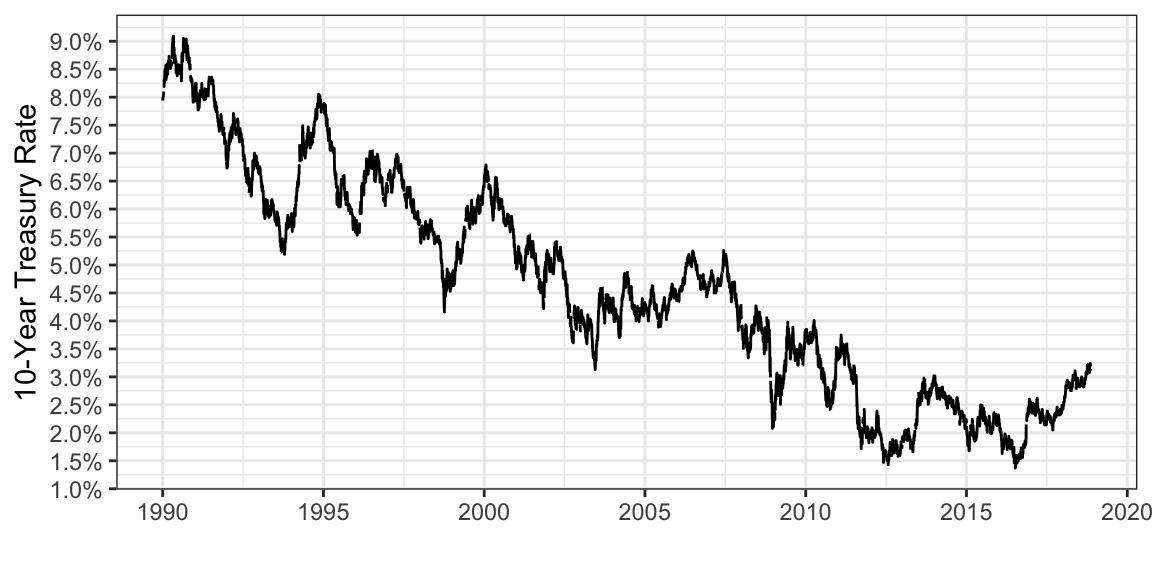
\includegraphics{bookdown-demo_files/figure-latex/unnamed-chunk-3-1} 

}

\caption{\label{fig::us-gdp-pce}\textsc{US GDP from NIPA (BEA)}}\label{fig:unnamed-chunk-3}
\end{figure}

To get a better of sense of how big consumption is as a fraction to GDP
(although you may eyeball it on this picture), we might plot consumption
as a function of GDP, which is what I do below. You can see that
Personal Consumption Expenditures are approximately \textbf{60 to 70 \%
of GDP}. You can also see that it's been rising since the end of the
sixties. We will discuss that.

\begin{figure}

{\centering 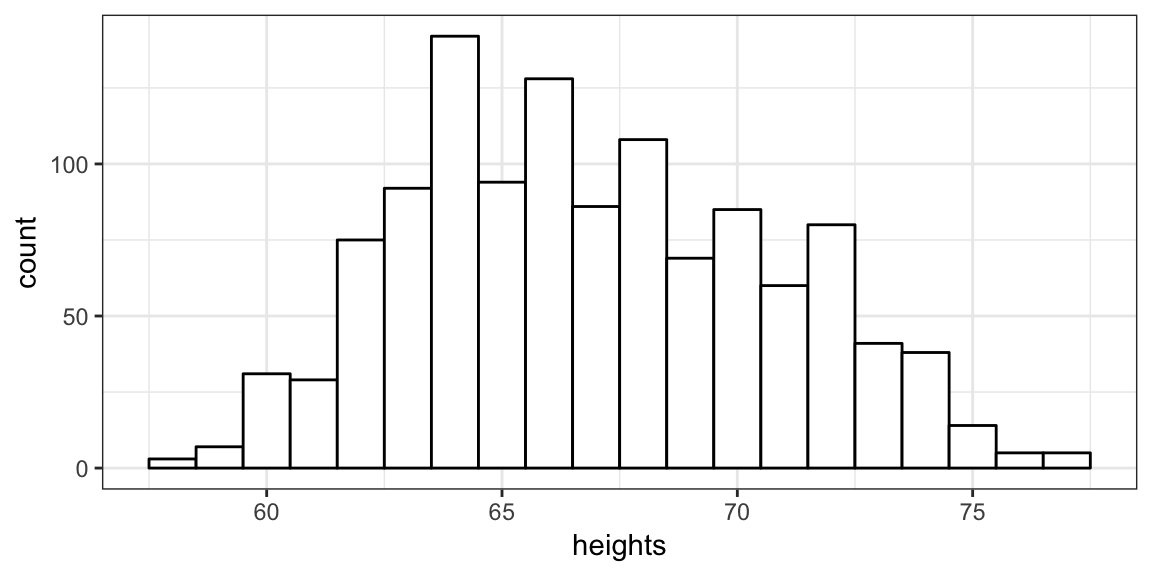
\includegraphics{bookdown-demo_files/figure-latex/unnamed-chunk-4-1} 

}

\caption{\label{fig::us-gdp}\textsc{Consumption as a share of GDP from NIPA (BEA)}}\label{fig:unnamed-chunk-4}
\end{figure}

Personal Consumption Expenditures are divided up into:

\begin{itemize}
\tightlist
\item
  Durable Goods (more than 3 years of durability): e.g.~cars.
\item
  Non-durable Goods (less than 3 years of durability).
\item
  Services.
\end{itemize}

Services have become more important than Goods in total consumption
since the 1970s.

\begin{figure}

{\centering 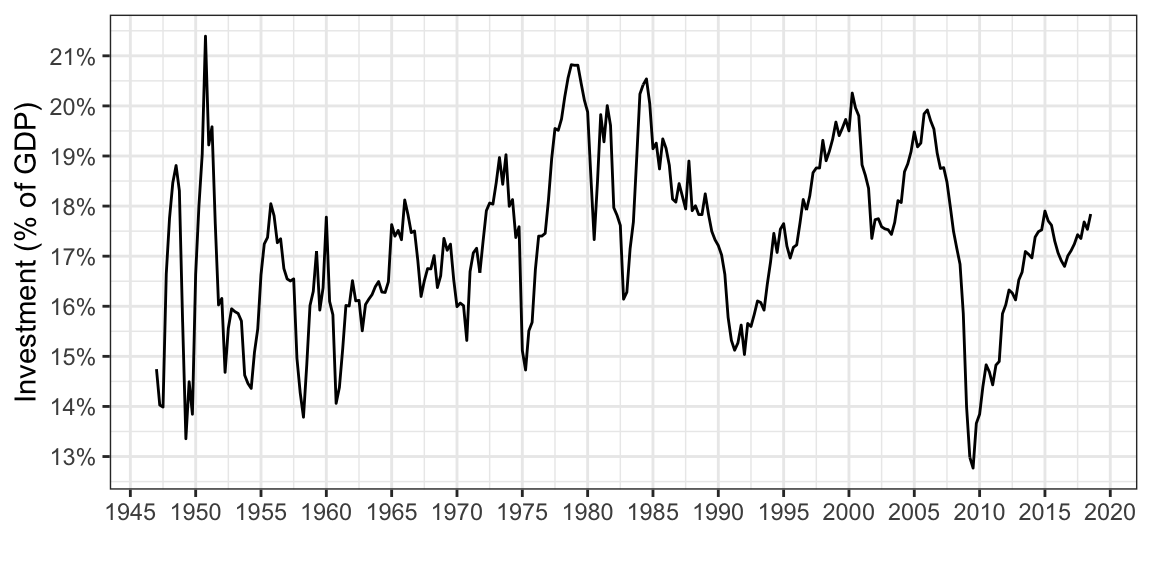
\includegraphics{bookdown-demo_files/figure-latex/unnamed-chunk-5-1} 

}

\caption{\label{fig::us-gdp}\textsc{Goods and Services Consumption as a share of GDP from NIPA (BEA)}}\label{fig:unnamed-chunk-5}
\end{figure}

\hypertarget{inv}{\subsection{Gross private domestic investment -
Investment (I)}\label{inv}}

Investment has two components:

\begin{itemize}
\tightlist
\item
  non residential investment is the purchase of new capital goods by
  firms: structures, new plants.
\item
  residential investment is the purchase of new houses.
\end{itemize}

Gross private domestic investment is approximately \textbf{15 to 20 \%
of GDP}, as you can see on Figure \ref{fig::us-capital-formation}. It is
also very volatile over the cycle.

\begin{figure}

{\centering 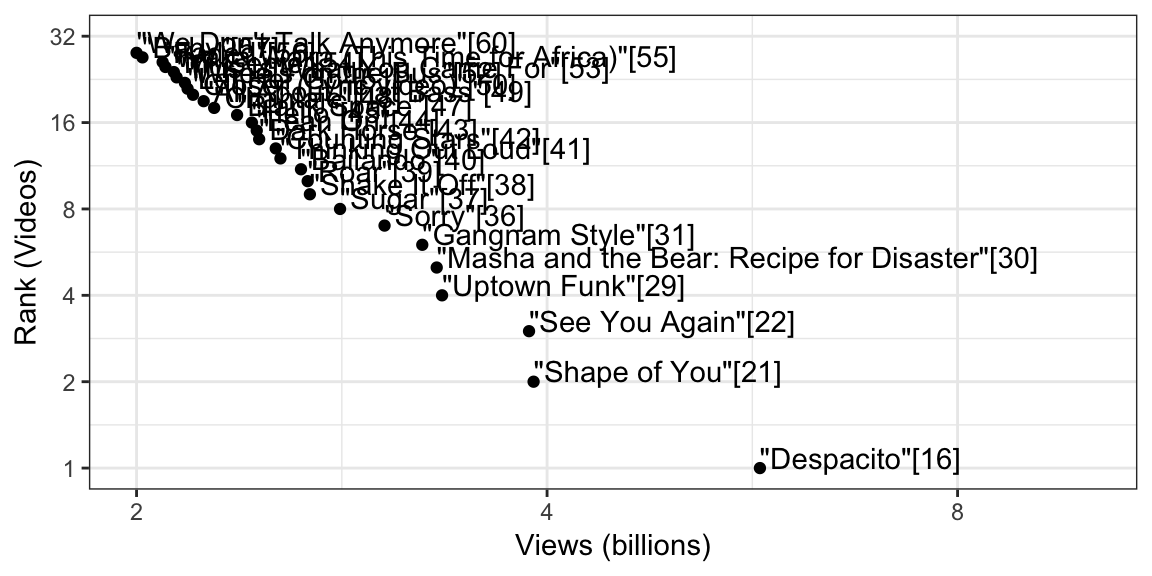
\includegraphics{bookdown-demo_files/figure-latex/unnamed-chunk-6-1} 

}

\caption{\label{fig::us-capital-formation}\textsc{Investment as a share of GDP from NIPA (BEA)}}\label{fig:unnamed-chunk-6}
\end{figure}

\hypertarget{gov}{\subsection{Government Purchases (G)}\label{gov}}

Government purchases are composed of purchases of goods by the
government plus the compensation of government employees. Overall, they
comprise about approximately 20\% of GDP, as can be seen on Figure
\ref{fig::us-G}. Note however that they do not include transfers from
the government of interest payments on government debt.

\begin{figure}

{\centering 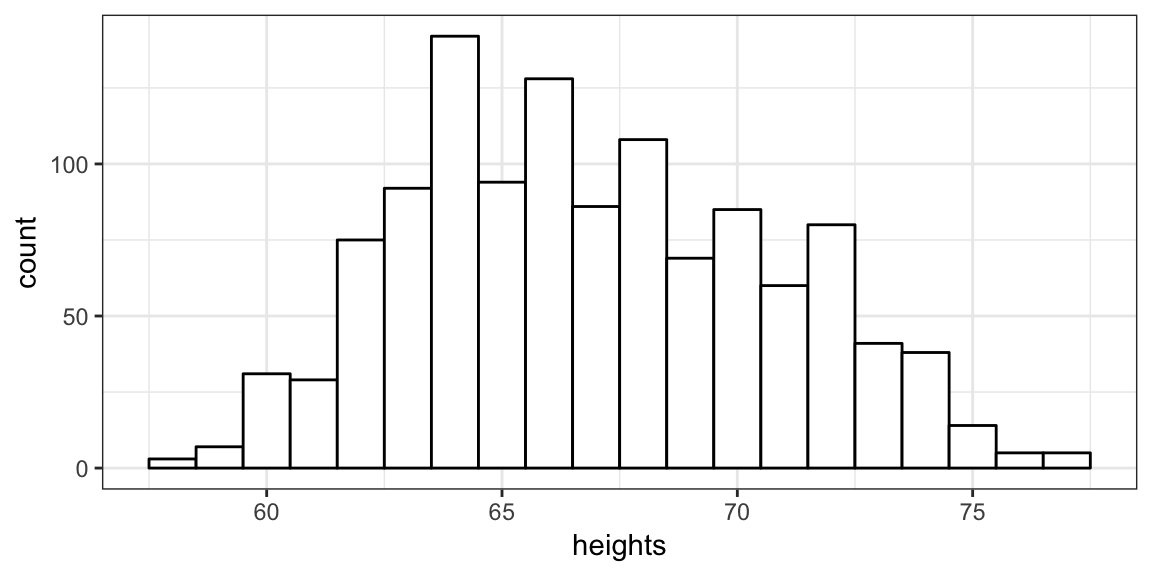
\includegraphics{bookdown-demo_files/figure-latex/unnamed-chunk-7-1} 

}

\caption{\label{fig::us-G}\textsc{Government Purchases as a share of GDP from NIPA (BEA)}}\label{fig:unnamed-chunk-7}
\end{figure}

\hypertarget{net-exports}{\subsection{Net Exports
(NX)}\label{net-exports}}

Net exports of goods and services are approximately \textbf{-2 to -6 \%
of GDP}, at least in the modern period (and in the United States), as
you can see on Figure \ref{fig::us-NX}.

\begin{figure}

{\centering 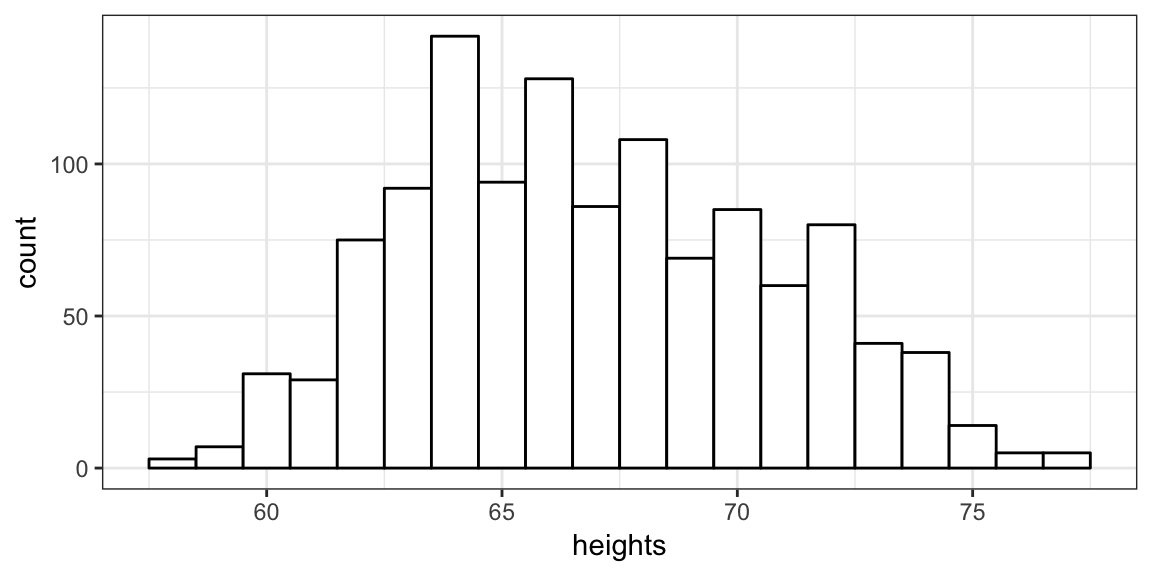
\includegraphics{bookdown-demo_files/figure-latex/unnamed-chunk-8-1} 

}

\caption{\label{fig::us-NX}\textsc{Net Exports as a share of GDP from NIPA (BEA)}}\label{fig:unnamed-chunk-8}
\end{figure}

\hypertarget{gdp-income}{\section{GDP: The Income
Approach}\label{gdp-income}}

\subsection{Cobb Douglas Production
function}\label{cobb-douglas-production-function}

In order to organize our thinking, let's write out a Cobb-Douglas
production function, defined as:
\[Y_t = A_t K_t^{\alpha} L_t^{1-\alpha},\] where \(\alpha\) is a number
between \(0\) and \(1\). It is useful to then think of a firm which
would choose the amount of labor it uses \(L_t\) as well as the amount
of capital it uses \(K_t\) in order to maximize its profits:
\[\max_{K_t, L_t} \quad A_t K_t^{\alpha} L_t^{1-\alpha} - R_t K_t - w_t L_t,\]
In this expression, \(R_t\) is the \textbf{rental rate} of capital, also
called the \textbf{gross return} to capital. This represents how much it
costs to rent one unit of capital. This cost actually has two
components:

\begin{enumerate}
\def\labelenumi{\arabic{enumi}.}
\item
  It includes a conventional interest rate \(r_t\), which is the cost of
  borrowing money to invest in capital. You should think of this as the
  real interest rate which is charged by a bank to borrow money.
\item
  It also includes a component to account for depreciation of the
  capital stock, often denoted by \(\delta\). If capital is bought, then
  the resale price for each unit of capital is lower by \(\delta\),
  which is a cost to the investor. If capital is rented, then capital
  needs to be given back to the owner in its original state.
\end{enumerate}

We have that the rental rate or gross return is equal to the net return
plus the depreciation rate: \[\boxed{R_t = r_t + \delta}.\] From Econ
11, it should be clear that a way to solve this problem is to set the
derivative of the profit function equal to \(0\) with respect to \(K_t\)
and \(L_t\):

\begin{itemize}
\tightlist
\item
  Differentiating with respect to \(K_t\) implies:
  \[\alpha A_t K_t^{\alpha-1} L_t^{1-\alpha} - R_t = 0 \quad \Rightarrow \quad \boxed{R_t = \alpha A_t K_t^{\alpha-1} L_t^{1-\alpha}}.\]
\item
  Differentiating with respect to \(L_t\) implies:
  \[(1-\alpha) A_t K_t^{\alpha} L_t^{-\alpha} - w_t = 0 \quad \Rightarrow \quad \boxed{w_t = (1-\alpha) A_t K_t^{\alpha} L_t^{-\alpha}}\]
\end{itemize}

Note that an alternative, and more direct way to get at that same
result, would be to use Econ 11 directly, and write that the marginal
products have to be equal to prices:

\begin{itemize}
\tightlist
\item
  The \textbf{rental rate of capital} \(R_t\) is the marginal product of
  capital. The marginal product of capital is how much more output is
  obtained when the capital stock is increased by one unit, which is
  just the derivative of output with respect to capital
  \(\partial Y_t / \partial K_t\): \[
  \begin{aligned}
  R_t&=\frac{\partial Y_t}{\partial K_t}\\
  &= \frac{\partial \left(A_t K_t^{\alpha} L_t^{1-\alpha}\right)}{\partial K_t}\\
  R_t &= \alpha A_t K_t^{\alpha-1} L_t^{1-\alpha}
  \end{aligned}
  \]
\item
  The \textbf{wage} \(w_t\) is the marginal product of labor. The
  marginal product of labor is how much more output is obtained when the
  quantity of labor is increased by one unit, which is just the
  derivative of output with respect to labor
  \(\partial Y_t / \partial L_t\): \[
  \begin{aligned}
  w_t &=\frac{\partial Y_t}{\partial L_t}\\
  &= \frac{\partial \left(A_t K_t^{\alpha} L_t^{1-\alpha}\right)}{\partial L_t}\\
  w_t &= (1-\alpha) A_t K_t^{\alpha} L_t^{-\alpha}
  \end{aligned}
  \] The total wage bill \(w L_t\) is a fraction \(1-\alpha\) of output
  \(Y_t\): \[
  \begin{aligned}
  w_t L_t &= (1-\alpha) A_t K_t^{\alpha} L_t^{-\alpha} \cdot L_t \\
  &= (1-\alpha) A_t K_t^{\alpha} L_t^{1-\alpha}\\
  w_t L_t &= (1-\alpha) Y_t
  \end{aligned}
  \]
\end{itemize}

The total capital income \(R_t K_t\) is a fraction \(\alpha\) of output
\(Y_t\): \[
\begin{aligned}
R_t K_t &= \alpha A_t K_t^{\alpha-1} L_t^{1-\alpha} \cdot K_t \\
&= \alpha A_t K_t^{\alpha} L_t^{1-\alpha}\\
R_t K_t &= \alpha Y_t.
\end{aligned}
\] This implies that the share of capital income in output (or
equivalently, value added) is: \[\frac{R_t K_t}{Y_t}=\alpha,\] while the
share of labor income in output (or equivalently, value added) is:
\[\frac{w_t L_t}{Y_t}=1-\alpha.\] Note that capital income plus labor
income equals total output: \[R_t K_t + w_t L_t = Y_t.\] Another way to
say the same thing is that the share of capital income in output and
that of labor income in output add up to one:
\[\boxed{\frac{R_t K_t}{Y_t} + \frac{w_t L_t}{Y_t}=1}.\]

\subsection{The Income Side in the
Data}\label{the-income-side-in-the-data}

In practice, how much goes to the compensation of employees (labor
income), and how much goes to the returns to capital (capital income)?
The answer is that it goes approximately for 1/3 to capital and for 2/3
to labor. In turn, this implies that we will, in numerical applications
of our theories, often assume that: \[\alpha = \frac{1}{3}\] The
calculations for these are less straightforward than for computing the
share of consumption, investment, as we did above. The reason is that in
practice, the division between labor and capital is not as clear cut in
the national accounts as one might hope: for example, someone who owns
her/his own business reports most of her/his income in the form of
capital income, even when a large part of it is actually labor income,
so that compensation of employees is (vastly) understated. Figure
\ref{fig::us-compensation-of-employees} shows which results are obtained
using this understated measure. It needs to be adjusted upwards by about
10\% of GDP, for the reasons mentioned above.

\begin{figure}

{\centering 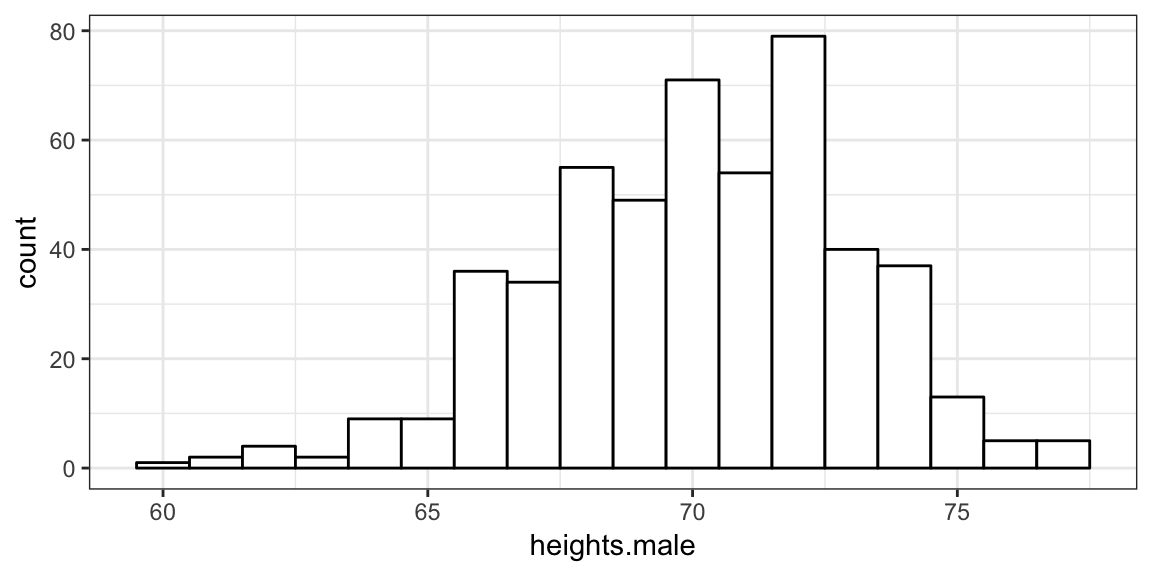
\includegraphics{bookdown-demo_files/figure-latex/unnamed-chunk-9-1} 

}

\caption{\label{fig::us-compensation-of-employees}\textsc{Compensation of Employees as a share of GDP from NIPA (BEA)}}\label{fig:unnamed-chunk-9}
\end{figure}

For our purposes, we only need to remember that the share of
compensation of employees is approximately 2/3 of value added.
Therefore, we will very often work with a Cobb-Douglas production
function such that: \[Y_t = A_t K_t^{1/3} L_t^{2/3}.\]
\href{lecture2.html}{Lecture 2} will walk you through the Solow growth
model, where we shall make heavy use of that Cobb-Douglas production
function.

\section*{Readings - To go further}\label{readings---to-go-further}
\addcontentsline{toc}{section}{Readings - To go further}

\href{https://hbr.org/2012/01/the-economics-of-well-being}{The Economics
of Well Being, \emph{Harvard Business Review}.}

\href{https://search.proquest.com/hnpnewyorktimes/docview/1030670685/A9EF0C9A254D4699PQ/1?accountid=14512}{G.D.P.
R.I.P., \emph{The New York Times}, August 9, 2009.}

(Gated)
\href{https://www.economist.com/news/finance-and-economics/21677223-new-study-shows-money-can-buy-you-happinessbut-only-fleetingly-others}{Keeping
up with the Karumes, \emph{The Economist}, October 29, 2015.}

(More Difficult Read)
\href{https://doi.org/10.1257/089533005774357833}{Abraham, Katharine G.
``Distinguished Lecture on Economics in Government-What We Don't Know
Could Hurt Us: Some Reflections on the Measurement of Economic
Activity.'' Journal of Economic Perspectives 19, no. 3 (September 2005):
3--18.}

\chapter{Solow Growth model}\label{solow-growth-model}

\section*{Introduction}\label{introduction}
\addcontentsline{toc}{section}{Introduction}

Robert Solow, 1987 Nobel Memorial Prize in Economic Sciences, starts
from a general production function, giving at any point in time output
\(Y_t\) as a function of inputs, capital \(K_t\) and labor \(L_t\):
\[Y_t=F\left(K_t,L_t\right).\]

\chapter{Two-period optimization
Problem}\label{two-period-optimization-problem}

\section{Introduction}\label{introduction-1}

Consumption and saving are perhaps the most important and controversial
issues in macroeconomics. In the Solow growth model, saving was a
constant fraction \(s\) of GDP, by assumption. We now build on
\emph{Economics 11} (the one where you learn consumer optimization with
Lagrangians and all that), in order to derive saving behavior from
microeconomic principles. In other words, we work to make saving
``endogenous'' (that is, explained by the model), while it was
previously taken as exogenous (that is, assumed in the model).

Although this discussion may appear somewhat abstract at first, these
calculations are the basis of some of the most important controversies
in macroeconomics, which we shall come to in the next lectures.

\section{The Two-Period Consumption
Problem}\label{the-two-period-consumption-problem}

\subsection{Assumptions}\label{assumptions}

There are two periods, \(t=0\) (think of this as ``today'') and \(t=1\)
(think of this as ``tomorrow''). The consumer values consumption \(c_0\)
in period \(0\) and \(c_1\) in period \(1\) according to the following
utility function:

\[U(c_{0},c_{1})=u(c_{0})+\beta u(c_{1}).\]

where \(u(.)\) is an increasing and concave function, and
\(\beta \leq 1\). \(\beta\) captures that people typically have a
preference for the present. (they are \textbf{present-biased})

Assume that agents earn (labor) income \(y_{0}\) in period \(0\), and
(labor) income \(y_{1}\) in period \(1\). They also are born with some
financial wealth \(f_{0}\) now, and have financial wealth \(f_{1}\) in
period 1, which they consume entirely because this is the last period.
(there is no point keeping more money for after period 1, because there
is no future at that point) The amount that agents save in this economy
is thus \(f_{1}-f_{0}\), and the amount of their accumulated savings is
the savings they already had plus what they decided to accumulate, so
that \(f_{0}+(f_{1}-f_{0})=f_{1}.\)

Therefore, consumption in period \(0\) is given by:

\[c_{0} =y_{0}-(f_{1}-f_{0})\]

The second period consumption \((t=1)\) is given by income plus the
return to (accumulated !) savings:

\[c_{1} =y_{1}+(1+r)f_{1}.\]

\subsection{Solution}\label{solution}

\textbf{Intertemporal budget constraint.} Rewriting \(f_{1}\) from this
second equation: \(f_{1}=(c_{1}-y_{1})/(1+r)\), and plugging into the
first,

\[c_{0}=y_{0}-\left(\frac{c_{1}-y_{1}}{1+r}-f_{0}\right).\] Rearranging,
total wealth is then the sum of financial wealth \(f_0\) and of the
present discounted value of human wealth:

\[c_{0}+\frac{c_{1}}{1+r}=\overbrace{f_{0}+\underbrace{y_{0}+\frac{y_{1}}{1+r}}_{\text{human wealth}}}^{\text{total wealth}}.\]

The intertemporal budget constraint says that the present discounted
value of consumption is equal to total wealth.

\textbf{Optimization.} The problem of the consumer is then simply that
of maximizing utility under his budget constraint:

\[
\begin{aligned} 
\max_{c_{0},c_{1}} & \quad u(c_{0})+\beta u(c_{1}) \\
& \text{s.t.} \quad c_{0}+\frac{c_{1}}{1+r}=f_{0}+y_{0}+\frac{y_{1}}{1+r}.
\end{aligned}
\]

You may solve this optimization in four different ways:

\begin{enumerate}
\def\labelenumi{\arabic{enumi}.}
\item
  Apply the well known ratio of marginal utilities formula from Econ 11.
  Let us rewrite this optimization problem as follows: \[
  \begin{aligned} 
  \max_{c_{0},c_{1}} & \quad u(c_{0})+\beta u(c_{1}) \\
  & \text{s.t.} \quad p_0c_{0}+p_1 c_1=B.
  \end{aligned}
  \] where we have defined the price of consumption in period \(0\) by:
  \[p_0 \equiv 1,\] the price of consumption in period \(1\) by:
  \[p_1 \equiv \frac{1}{1+r},\] and finally the budget \(B\) by the
  present discounted value of lifetime resources:
  \[B \equiv f_{0}+y_{0}+\frac{y_{1}}{1+r}.\] Note that the relative
  price of consumption in period \(1\) relative to period \(0\) is given
  by \(1/(1+r)\): when the interest rate becomes higher, consuming in
  period \(1\) becomes relatively cheaper, or consuming in period \(0\)
  becomes more expensive (it's really expensive to consume now rather
  than later if the bank is offering me a really high interest rate).
  Thus, applying the formula from Econ 11 allows to say that the
  marginal rate of substitution between consumption in period \(1\)
  \(c_1\) and consumption in period \(0\) \(c_0\) - the ratio of
  marginal utilities - is equal to the ratio of prices:
  \[\frac{\partial U / \partial c_1}{\partial U / \partial c_0} = \frac{p_1}{p_0}= \frac{1}{1+r} \quad\Rightarrow\quad\frac{\beta u'(c_{1})}{u'(c_{0})}=\frac{1}{1+r}.\]
\item
  Apply the following intuitive economic argument. The marginal utility
  from consuming in period \(1\) is \(\beta u'(c_{1})\). The marginal
  utility from consuming in period \(0\) is \(u'(c_{0})\). By putting
  one unit of consumption in the bank, one forgoes \(1\) unit of
  consumption in period \(0\) to get \(1+r\) units of consumption in
  period \(1\). The two have to be equal, if one is optimizing. If
  consuming more in period \(0\) gives a higher marginal utility, or
  \(u'(c_{0})>(1+r)\beta u'(c_{1})\), then one should consume more and
  save less. On the contrary, should \(u'(c_{0})<(1+r)\beta u'(c_{1})\),
  one should consume less and save more. Therefore, in equilibrium,
  these two options can only be equal:
  \[u'(c_{0})=(1+r)\beta u'(c_{1})\quad\Rightarrow\quad\frac{\beta u'(c_{1})}{u'(c_{0})}=\frac{1}{1+r}.\]
\item
  Replace \(c_{0}\) from the intertemporal budget constraint above and
  optimize with respect to \(c_{1}\):
  \[\max_{c_{1}}\quad u\left[\left(f_{0}+y_{0}+\frac{y_{1}}{1+r}\right)-\frac{c_{1}}{1+r}\right]+\beta u(c_{1}).\]
  Taking the derivative of this expression with respect to \(c_1\) leads
  to: \[
  \begin{aligned}
  &-\frac{1}{1+r} u'\left[\left(f_{0}+y_{0}+\frac{y_{1}}{1+r}\right)-\frac{c_{1}}{1+r}\right]+\beta u'(c_{1})=0\\
  &\quad\Rightarrow\quad-\frac{1}{1+r}u'(c_{0})+\beta u'(c_{1})=0\quad\Rightarrow\quad\frac{\beta u'(c_{1})}{u'(c_{0})}=\frac{1}{1+r}.
  \end{aligned}
  \] where the first substitution uses the intertemporal budget
  constraint which implies: \[
  \begin{aligned}
  \left(f_{0}+y_{0}+\frac{y_{1}}{1+r}\right)-\frac{c_{1}}{1+r}=c_0
  \end{aligned}
  \]
\item
  Alternatively, you may substitute \(c_{1}\) out and optimize with
  respect to \(c_{0}\): \[
  \begin{aligned}
  \max_{c_{0}}\quad u(c_{0})+\beta u\left[(1+r)\left(f_{0}+y_{0}+\frac{y_{1}}{1+r}\right)-(1+r)c_{0}\right].
  \end{aligned}
  \] Taking the derivative of this expression with respect to \(c_0\)
  leads to: \[
  \begin{aligned}
  &u'(c_{0})-\beta(1+r)u'\left[(1+r)\left(f_{0}+y_{0}+\frac{y_{1}}{1+r}\right)-(1+r)c_{0}\right]=0\\
  &\quad\Rightarrow\quad u'(c_{0})-\beta(1+r)u'(c_{1})=0\quad\Rightarrow\quad\frac{\beta u'(c_{1})}{u'(c_{0})}=\frac{1}{1+r}.
  \end{aligned}
  \] where the first substitution uses the intertemporal budget
  constraint which implies (pre-multiplying both sides by \(1+r\)): \[
  \begin{aligned}
  (1+r)\left(f_{0}+y_{0}+\frac{y_{1}}{1+r}\right)-(1+r)c_{0}=c_1
  \end{aligned}
  \]
\end{enumerate}

\subsection{Some examples}\label{some-examples}

\textbf{Log utility, no discounting (\(\beta = 1\)).} Log utility
implies that \(u(c)\) is given by the natural logarithm. Marginal
utility is then just: \[u'(c)=\frac{1}{c},\]

Since \(\beta=1\), the above optimality condition (derived 4 times) can
be written as: \[
\begin{aligned}
& \frac{u'(c_{1})}{u'(c_{0})}=\frac{1}{1+r} \quad \Rightarrow \quad \frac{1/c_1}{1/c_0}=\frac{1}{1+r} \\
& \quad \Rightarrow \quad \frac{c_0}{c_1}=\frac{1}{1+r} \quad \Rightarrow \quad c_{0}=\frac{c_{1}}{1+r}
\end{aligned}
\] Substituting out \(c_{1}/(1+r)=c_0\) in the intertemporal budget
constraint allows to calculate consumption at time \(0\) \(c_0\): \[
\begin{aligned}
&c_{0}+\frac{c_{1}}{1+r}=f_{0}+y_{0}+\frac{y_{1}}{1+r}\\
&\quad \Rightarrow \quad c_{0}+c_0=f_{0}+y_{0}+\frac{y_{1}}{1+r}\\
&\quad \Rightarrow \quad c_{0}=\frac{1}{2}\left(f_{0}+y_{0}+\frac{y_{1}}{1+r}\right)
\end{aligned}
\] Finally, we may calculate \(c_1\): \[
\begin{aligned}
c_{1}&=(1+r)c_0=\frac{1+r}{2}\left(f_{0}+y_{0}+\frac{y_{1}}{1+r}\right).
\end{aligned}
\]

According to this expression, the \textbf{Marginal Propensity to Consume
(MPC)} out of current wealth \(f_{0}\) is given by \(1/2\). When \(f_0\)
rises to \(f_0+\Delta f_0\), the corresponding change in consumption is:
\[\Delta c_0 = \frac{1}{2}\Delta f_0.\] If we were to study a model with
more periods, say \(T\) periods, we would find that people Marginal
Propensity to Consume is approximately equal to \(1/T\), at least
according to this model. Whether such is actually the case, and people
are that rational, is a subject of fierce debate among macroeconomists,
and one that we will take up in the next lectures.

\textbf{Log utility, with discounting (\(\beta < 1\)).} Marginal utility
is then \(u'(c)=1/c\), so that the optimality condition gives: \[
\begin{aligned}
& \frac{\beta u'(c_{1})}{u'(c_{0})}=\frac{1}{1+r} \quad \Rightarrow \quad \frac{\beta/c_1}{1/c_0}=\frac{1}{1+r} \\
& \quad \Rightarrow \quad \frac{\beta c_0}{c_1}=\frac{1}{1+r} \quad \Rightarrow \quad \beta c_{0}=\frac{c_{1}}{1+r}
\end{aligned}
\] Substituting out \(c_{1}/(1+r)=\beta c_0\) in the intertemporal
budget constraint allows to calculate consumption at time \(0\) \(c_0\):
\[
\begin{aligned}
&c_{0}+\frac{c_{1}}{1+r}=f_{0}+y_{0}+\frac{y_{1}}{1+r}\\
&\quad \Rightarrow \quad c_{0}+\beta c_0=f_{0}+y_{0}+\frac{y_{1}}{1+r}\\
&\quad \Rightarrow \quad c_{0}=\frac{1}{1+\beta}\left(f_{0}+y_{0}+\frac{y_{1}}{1+r}\right)
\end{aligned}
\] Finally, we may calculate \(c_1\): \[
\begin{aligned}
c_{1}&=\beta (1+r)c_0=\frac{\beta(1+r)}{1+\beta}\left(f_{0}+y_{0}+\frac{y_{1}}{1+r}\right).
\end{aligned}
\]

Because people are more impatient in this case, they consume more, and
their Marginal Propensity to Consume (MPC) is \textbf{higher} with
\(\beta<1\): \[\Delta c_0 = \frac{1}{1+\beta}\Delta f_0.\]

Note that the solution with no discounting corresponds to that with
discounting when \(\beta=1\), which was expected.

\subsection{Generalization}\label{generalization}

Assume that an individual receives wage \(w\) in period \(0\), and that
this wage is expected to grow at rate \(g\) in the next \(T\) years.
What is the present value of his human wealth, assuming that the
interest rate is given by \(R\)? The answer is that his human wealth
\(H\) is given as follows:

\[H =w+w\frac{1+g}{1+r}+w\left(\frac{1+g}{1+r}\right)^{2}+...+w\left(\frac{1+g}{1+r}\right)^{T-1}\]

\[H =w\frac{1-\left(\dfrac{1+g}{1+r}\right)^{T}}{1-\dfrac{1+g}{1+r}}\]

\chapter{Applications}\label{applications}

Some \emph{significant} applications are demonstrated in this chapter.

\section{Example one}\label{example-one}

\section{Example two}\label{example-two}

\chapter{Final Words}\label{final-words}

We have finished a nice book.

\bibliography{book.bib,packages.bib}


\end{document}
